\documentclass[12pt, a4paper]{report}
\usepackage{graphicx} %LaTeX package to import graphics
\usepackage[shortlabels]{enumitem}
\usepackage{geometry}
\usepackage{xcolor}
\geometry{lmargin=30mm}
\usepackage[export]{adjustbox}
\usepackage{titlesec}
\usepackage{float}
\usepackage{listings}

\usepackage{hyperref}

\titleformat{\chapter}{\normalfont\huge}{\thechapter}{20pt}{\huge\bf}
\graphicspath{{images/}} %configuring the graphicx package
\title{Practica 3}
\author{Javier Izquierdo Hernández}
\date{\today}
\begin{document}
	\begin{titlepage}
		\centering
		{
\includegraphics[width=0.3\textwidth]{logo}\par}
		\vspace{1cm}
		{\bfseries\LARGE Universidad Rey Juan Carlos \par}
		\vspace{1cm}
		{\scshape\Large E.T.S. Ingeniería de Telecomunicación \par}
		\vspace{3cm}
		{\scshape\Huge Redes de Ordenadores para Robots y Máquinas Inteligentes \par}
		\vspace{3cm}
		{\itshape\Large Práctica 3 \par}
		\vfill
		{\Large Autor: \par}
		{\Large Javier Izquierdo Hernández \par}
		\vfill
		{\Large \today \par}
	\end{titlepage}

\newpage
\renewcommand{\contentsname}{Contenidos}
\tableofcontents
\newpage

Antes de comenzar, descarga tu escenario del siguiente enlace donde deberás introducir tu número
de DNI (8 dígitos) con la letra correspondiente:\\
\begin{center}
https://mobiquo.gsyc.urjc.es/practicas/ror/p3.html	
\end{center}

En la figura 1 se representa un conjunto de subredes y máquinas (pc1, pc2, pc4, pc5, r1, r2 y
firewall) que pertenecen a una determinada empresa y su conexión a Internet a través de la máquina
firewall. La empresa tiene definidas un conjunto de subredes de ámbito privado:\\
\begin{itemize}
	\item 10.X.0.0/24: r1(eth1), pc1, pc2
	\item 10.X.1.0/24: firewall(eth0), r1(eth0), r2(eth0)
	\item 10.X.2.0/24: r2(eth1), pc3
\end{itemize}

Adicionalmente, la empresa tiene las máquinas pc4 y pc5 que se encuentran en una subred pública: 100.X.0.0/24. Estas máquinas proporcionan servicios básicos de la empresa: servidor de HTTP y
servidor de fecha y hora. A esta zona de la red interna donde la empresa tiene una o varias subredes
públicas para ofrecer servicios a Internet se le denomina zona desmilitarizada o DMZ (DeMilitarized
Zone).\\

Todas las máquinas de la empresa se conectan a Internet a través de la máquina firewall y la
subred 100.X.1.0/24.\\

En este escenario, se considera que Internet está formado por las siguientes máquinas: r3, r4, r5,
pc6 y pc7 que se encuentran conectadas a las siguientes subredes públicas:
\begin{itemize}
	\item 100.X.1.0/24: r3(eth0)
	\item 100.X.2.0/24: r3(eth1), r5(eth2)
	\item 100.X.3.0/24: r3(eth2), r4(eth2)
	\item 100.X.4.0/24: r4(eth1), r5(eth0)
	\item 100.X.5.0/24: r4(eth0), pc6
	\item 100.X.6.0/24: r5(eth1), pc7
\end{itemize}
Arranca de una en una todas las máquinas de la figura.
\begin{figure}[h]
	\centering
	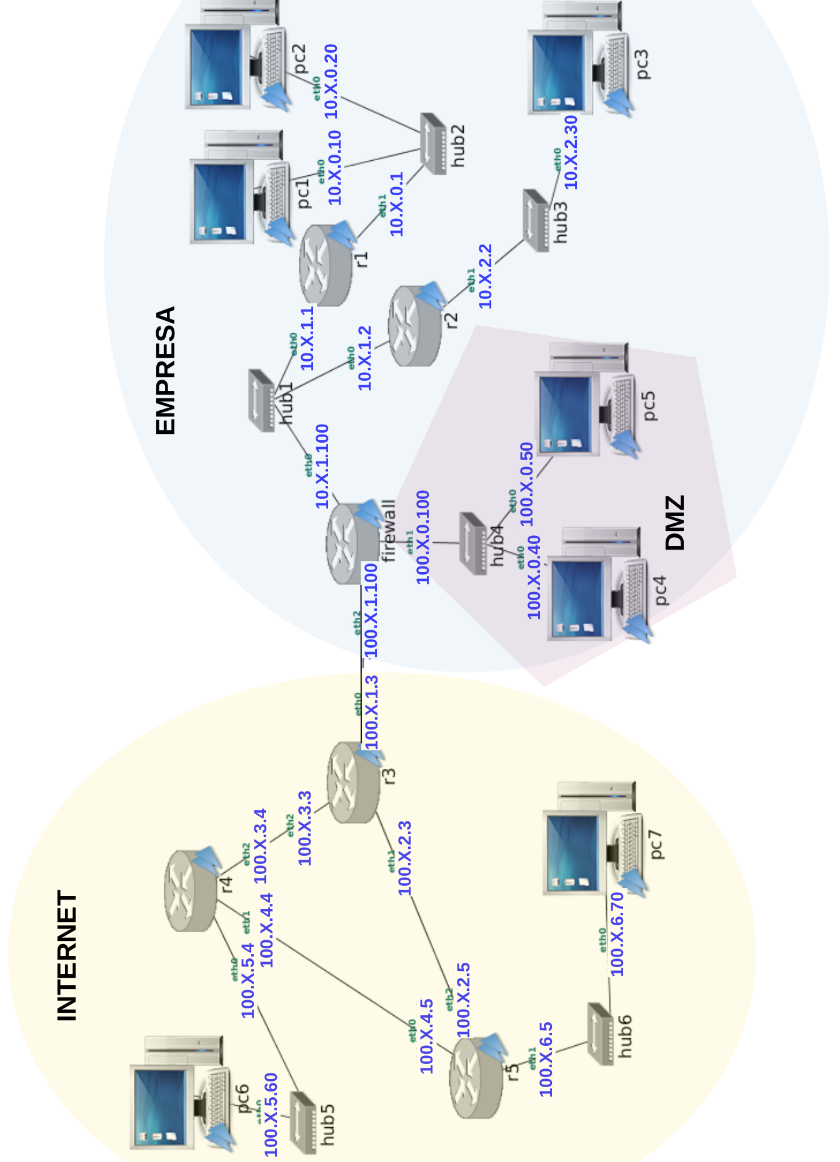
\includegraphics[width=0.8\textwidth,rotate=-90]{enunciado1}
	\caption{Escenario de red para la configuración de un firewall}
\end{figure}
\chapter{Introducción}
A continuación se proporcionan algunos consejos para facilitar la realización de la práctica.
\section{Edición y ejecución de scripts}
En esta práctica se configurará la máquina firewall para que actúe como traductor de direcciones y como cortafuegos. Habrá que definir varias reglas utilizando iptables. Por este motivo, es
recomendable guardar dichas reglas en un fichero script de shell.\\

Considera la posibilidad de editar y guardar el script en el sistema de ficheros de la máquina real,
ejecutándolo desde dentro de la máquina virtual. Así, si tu script fw.sh está almacenado directamente
en tu HOME de la máquina real, podrías editarlo en ella con un editor gráfico (por ejemplo, gedit) y
luego ejecutarlo en la máquina firewall escribiendo dentro de esa máquina virtual:
\begin{center}
\textbf{/hosthome/fw.sh}
\end{center}

\section{Comprobación de la configuración del \textit{firewall}}
Durante la práctica frecuentemente tendrás que ir comprobando que el firewall está correctamente
configurado, es decir:
\begin{itemize}
	\item deja pasar el tráfico que está permitido.
	\item impide el paso del tráfico que debe ser bloqueado.
	\item realiza la traducción de direcciones IP necesaria para que no aparezcan en Internet paquetes con
	direcciones privadas
\end{itemize}
Para ello deberás emplear la herramienta netcat (nc) (ya utilizada en prácticas del curso pasado)
que permite arrancar aplicaciones TCP y UDP en modo cliente o servidor.\\

El enunciado de la práctica te irá indicando cuándo y en qué máquinas debes lanzar un cliente o
un servidor TCP o UDP para ir probando la configuración del firewall. Consulta la documentación
adjunta para recordar la sintaxis de netcat.\\

\chapter{Traducción de direcciones y puertos en el firewall: tabla nat}
\section{Clientes en la red privada, servidores externos}
Configura un script \textbf{fw1.sh} en el \textit{firewall} para que:
\begin{itemize}
	\item se borren las reglas que hubiera configuradas previamente en la tabla \textbf{nat}
	\item se reinicien los contadores de la tabla \textbf{nat}
	\item se realice la traducción de direcciones para el tráfico saliente de las redes privadas (SNAT) y su
	correspondiente tráfico de respuesta.
\end{itemize}
Incluye el script en la memoria. Ver el script en \ref{fw1}.
\subsection{Pruebas con TCP}
Ejecuta el script \textbf{fw1.sh} de 2.1.
\begin{enumerate}
	\item Captura el tráfico en \textbf{r3-eth0} (\textcolor{blue}{iptables-01.cap}) y en \textbf{firewall-eth0} (\textcolor{blue}{iptables-02.cap}) para
	ver los paquetes dentro de la red de la Empresa y por Internet. Arranca las siguientes aplicaciones:
	\begin{itemize}
		\item nc como servidor TCP en pc6, puerto 7777
		\item nc como cliente TCP en pc1
	\end{itemize}
	Sin escribir nada ni en el cliente ni en el servidor, consulta la información de\textbf{ ip\_conntrack}
	del \textbf{firewall} cada medio segundo. Para hacerlo automáticamente, en vez de repetir el comando
	utiliza watch de la siguiente forma:
	\begin{center}
		firewall:$\sim$\# watch -n 0.5 cat /proc/net/ip\_conntrack
	\end{center}
	Explica el número de paquetes que se han observado en cada sentido, razonando la respuesta,
	indicando de qué paquetes se trata (recuerda que estamos ante una conexión TCP).\\
	
	Se han mandado dos mensajes desde pc1 a pc6, el mensaje de Syn para abrir la conexión y el mensaje de Ack a la respuesta al primer mensaje de pc6.\\
	Y en la dirección contraria se habrá mandado 1 solo mensaje que será la respuesta a la apertura de la conexión.
	\begin{figure}[h]
		\centering
		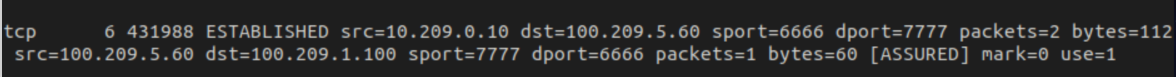
\includegraphics[width=0.8\textwidth]{ej2.1.1_1}
	\end{figure}
	\item Introduce una palabra en la entrada estándar de pc1, pulsa $<$Enter$>$ y observa los cambios en
	\textbf{ip\_conntrack}. Explica a qué se deben.\\
	
	El tiempo que le queda a la conexión se resetea a 120 horas o 432000 segundos porque se recibe un paquete.
	\begin{figure}[h]
		\centering
		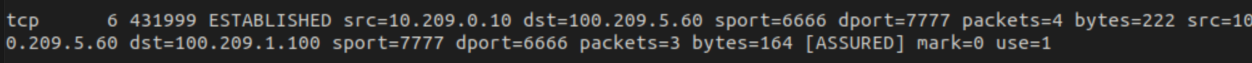
\includegraphics[width=0.8\textwidth]{ej2.1.1_2}
	\end{figure}
	\item Realiza un Ctrl+C en el terminal de \textbf{pc1} para interrumpir la ejecución de \textbf{nc}. Observa los cambios
	en \textbf{ip\_conntrack }y explica a qué se deben.\\
	
	El tiempo que le queda a la conexión desciende a 120 segundos y la conexión pasa a tener el valor de TIME\_WAIT ya que esa conexión ha sido cerrada tanto por el cliente como por el servidor, entonces no tiene sentido recordarla.
	\begin{figure}[h]
		\centering
		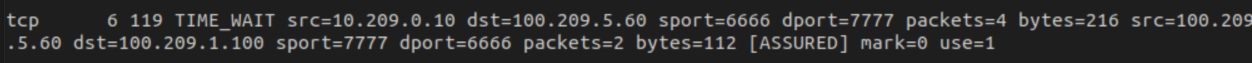
\includegraphics[width=0.8\textwidth]{ej2.1.1_3}
	\end{figure}
	\item Interrumpe las capturas, y estúdialas. En particular, identifica los mismos paquetes en las 2
	capturas, y observa cómo cambian las direcciones IP de los mismos paquetes según viajen dentro
	de la EMPRESA o por INTERNET. Explica el resultado.\\
	
	En la captura dentro de la empresa en la interfaz eth0 del firewall se puede ver que los mensajes van de la dirección Ip de pc1 a la de pc6 y viceversa, sin ninguna traducción.\\
	Mientras que en la captura en Internet los mensajes se intercambian entre pc6 y la dirección Ip del firewall que da con Internet, es decir, que la dirección Ip de pc2 no aparece en ningún momento.
	\item Consulta la lista de reglas en el firewall con:
	\begin{center}
		firewall:$\sim$\# iptables -t nat -L -v -n
	\end{center}
	Obseva qué regla(s) están cumpliendo los paquetes y cuántas veces se cumple(n).\\
	
	Se está cumpliendo la única regla que hemos añadido
	\begin{center}
		\begin{itemize}
			\item iptables -t nat -A POSTROUTING -s 10.209.0.0/16 -o eth2 -j SNAT --to-source 100.209.1.100
		\end{itemize}
	\end{center}
	1 vez.
	\begin{figure}[h]
		\centering
		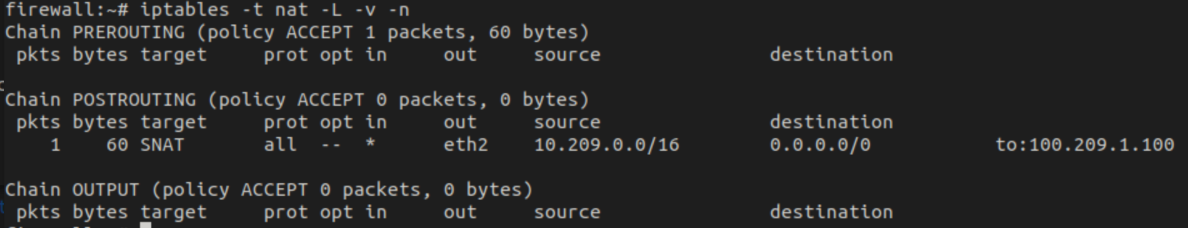
\includegraphics[width=0.8\textwidth]{ej2.1.1_5}
	\end{figure}
	\item Vuelve a repetir la misma prueba anterior (sin necesidad de realizar las capturas de tráfico): lanza
	servidor y cliente, intercambia tráfico, y termina la conexión. Vuelve a mirar qué regla(s) se están
	cumpliendo y \textbf{cuántas veces} se cumple(n).\\
	
	Se cumple 2 veces la misma regla que en el apartado anterior, el de la primera captura y el del inicio de la segunda conexión.\\
	\begin{figure}[h]
		\centering
		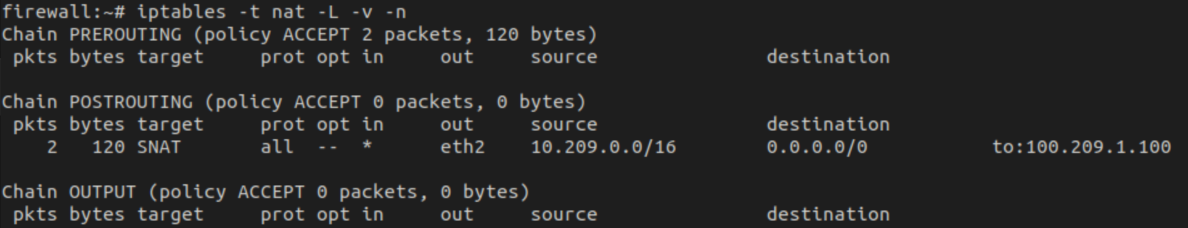
\includegraphics[width=0.8\textwidth]{ej2.1.1_6}
	\end{figure}
\end{enumerate}
\subsection{Pruebas con UDP}
Ejecuta el script \textbf{fw1.sh} de 2.1 para que se reinicien los contadores de paquetes de iptables, compruébalo consultando la lista de reglas del firewall.
\begin{enumerate}
	\item Captura el tráfico en \textbf{r3-eth0} (\textcolor{blue}{iptables-03.cap}) y en \textbf{firewall-eth0} (\textcolor{blue}{iptables-04.cap}) para
	ver los paquetes dentro de la red de la Empresa y por Internet. Arranca las siguientes aplicaciones:
	\begin{itemize}
		\item \textbf{nc} como servidor UDP en \textbf{pc6}, puerto 7777
		\item \textbf{nc} como cliente UDP en \textbf{pc2}
	\end{itemize}
	Realiza las siguientes pruebas:
	\begin{enumerate}[a)]
		\item Sin escribir nada ni en el cliente ni en el servidor, consulta la información de \textbf{ip\_conntrack}
		del \textbf{firewall} cada medio segundo. Recuerda que el tráfico es ahora UDP y no hay conexiones
		propiamente dichas. Explica el resultado.\\
		No hay nada, porque al no escribir no se inicia una conexión.
		\item Escribe 5 líneas en el terminal de \textbf{pc2} para que se las envíe a \textbf{pc6}. Explica el número de
		paquetes enviados en la información que muestra \textbf{ip\_conntrack}.\\
		Ip\_conntrack muestra 5 paquetes.\\
		\begin{figure}[h]
			\centering
			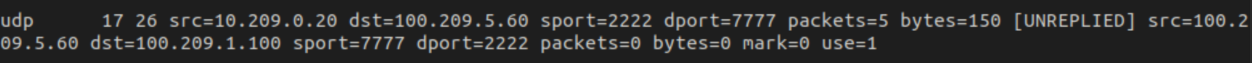
\includegraphics[width=0.8\textwidth]{ej2.1.2_1.b}
		\end{figure}
		\item Escribe una línea en \textbf{pc6 }para que se la envíe a \textbf{pc2}. Explica nuevamente el número de
		paquetes en \textbf{ip\_conntrack}.\\
		
		Si pc6 envía el mensaje antes de que pasen los 30 segundos necesarios para que el firewall olvide la asociación aparecerán 5 paquetes como anteriormente en la "primera" parte, mientras que aparecerá un paquete en la otra.\\
		Si pasan los 30 segundos el servidor se cerrará al dar error en la conexión.\\
		\begin{figure}[h]
			\centering
			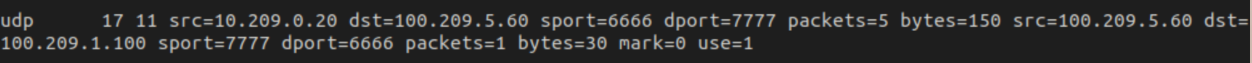
\includegraphics[width=0.8\textwidth]{ej2.1.2_1.c}
		\end{figure}
		\item Observa el poco tiempo que se mantiene la “asociación” entre cliente y servidor en \textbf{ip\_contrack}.
		Indica cuánto ha sido.\\
		Han sido 30 segundos.
		\item Interrumpe la captura y las ejecuciones de \textbf{nc}, explica la captura y cómo ésta se relaciona
		con la información que has visto en \textbf{ip\_conntrack}.\\
		
		En r3 se puede ver que los datagramas Udp tienen la Ip de origen como 100.209.1.100 que es la del firewall al igual que en la segunda línea que se ve en la imagen superior en ip\_conntrack. Mientras que en eth0 del firewall se pueden ver que los mensajes serán entre las direcciones Ip mostradaas en la primera línea.\\
		También se aprecia que han habido 5 mensajes desde pc2 a pc6 y que pc6 ha contestado a pc2 1 vez, esto se ve en ip\_conntrack en el número de paquetes en cada "sentido".
	\end{enumerate}
	\item Consulta la lista de reglas en el \textbf{firewall}, e indica cuáles se están cumpliendo y cuántas veces
	se cumplen.\\
	
	Se está cumpliendo la única regla que hemos añadido
	\begin{center}
		\begin{itemize}
			\item iptables -t nat -A POSTROUTING -s 10.209.0.0/16 -o eth2 -j SNAT --to-source 100.209.1.100
		\end{itemize}
	\end{center}
	1 vez.
	\begin{figure}[h]
		\centering
		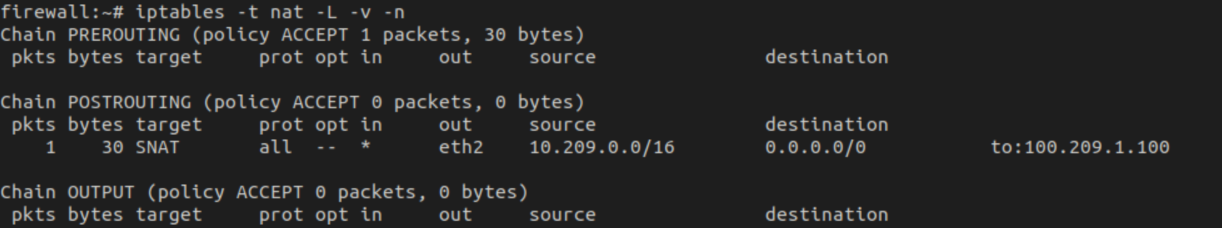
\includegraphics[width=0.8\textwidth]{ej2.1.2_2}
	\end{figure}
	\item Interrumpe la ejecución de cliente y servidor e inicia una nueva comunicación entre un nuevo
	cliente y un servidor UDP e intercambia tráfico entre ellos para ver cómo evolucionan las cuentas
	en la lista de reglas. Explica qué reglas se están cumpliendo ahora y \textbf{cuántas veces} se cumplen.\\
	
	Se cumple la misma regla que en el anterior y el número de veces dependerá de cada cuanto se mandes los mensajes desde pc2, ya que si se mandan antes de los 30 segundos no contarán, pero en caso contrario incrementará en 1 el contador.\\
	\begin{figure}[h]
		\centering
		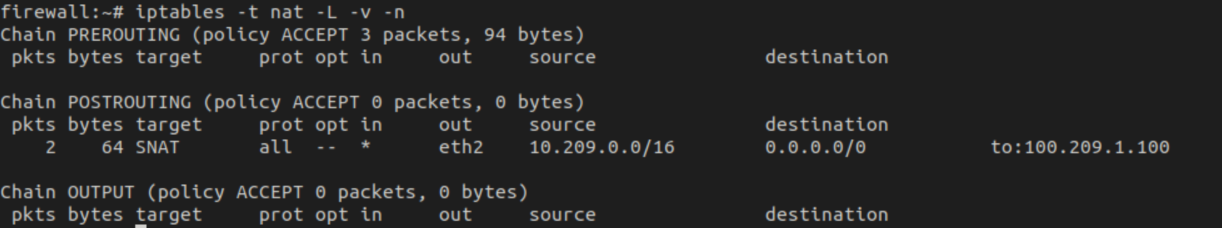
\includegraphics[width=0.8\textwidth]{ej2.1.2_3}
	\end{figure}
	\item Captura de nuevo el tráfico en \textbf{r3-eth0} (\textcolor{blue}{iptables-05.cap}) y en \textbf{firewall-eth0} (\textcolor{blue}{iptables-06.cap})
	para ver los paquetes dentro de la red de la Empresa y por Internet cuando tienes varios clientes
	desde un mismo puerto origen conectándose a un mismo servidor, para ello inicia:
	\begin{itemize}
		\item \textbf{nc} como servidor UDP en \textbf{pc7}, puerto 7777
		\item \textbf{nc} como cliente UDP en \textbf{pc1}, puerto 6666
		\item \textbf{nc} como cliente UDP en \textbf{pc2}, puerto 6666
	\end{itemize}
	Ahora, envía una línea desde \textbf{pc1} y después una línea desde \textbf{pc2}. Ten en cuenta que \textbf{nc} no funciona
	como las aplicaciones servidoras que pueden atender a varios clientes a la vez. La aplicación \textbf{nc}
	no está preparada para que un servidor se pueda comunicar a la vez con dos clientes, por ello el
	envío desde \textbf{pc2} provocará que \textbf{pc7} envíe un ICMP de error a \textbf{pc2}. Pero para lo que queremos
	comprobar este error no es importante, sólo queremos analizar lo que ocurre en el \textbf{firewall} con
	la traducción de direcciones IP y puertos.\\
	
	Interrumpe las capturas y analízalas fijándote en las direcciones IP y \textbf{puertos} que se utilizan en
	la red de la EMPRESA y en INTERNET.\\
	
	En la interfaz eth0 del firewall se reciben los 2 mensajes udp de pc1 y pc2 con sus Ip originales como origen y la Ip de pc7 como destino, y también con sus puertos originales. También esta presente el datagrama Icmp que envía pc7 al dar error, y este mantiene los mismo puertos que el mensaje original de pc2.\\
	Mientras tanto en r3 se puede ver que las Ip son reemplazadas por la del router que da a Internet y que el puerto del mensaje de pc2 ha cambiado a 1024 en vez de 6666, ya que este coincidía con el que tenía asignado anteriormente pc1. Lo mismo pasa para el mensaje de error, que va dirigido a la Ip del router y el puerto 1024.
\end{enumerate}
\subsection{Pruebas con ICMP}
Ejecuta el script \textbf{fw1.sh} de 2.1 para que se reinicien los contadores de paquetes de iptables. Vamos
a generar tráfico ICMP.
\begin{enumerate}
	\item Realiza una captura en \textbf{pc6} (\textcolor{blue}{iptables-07.cap}) y otra en \textbf{r1(eth1)} (\textcolor{blue}{iptables-08.cap}).
	\item Ejecuta el siguiente comando en \textbf{pc1} (recuerda sustituir la X por el número que te corresponde):
	\begin{center}
		pc1:$\sim$\# ping -c 2 100.X.5.60
	\end{center}
	\item Interrumpe las capturas anteriores.
	\item Consulta la información de \textbf{ip\_conntrack }del \textbf{firewall}. Verás que no aparece nada. Recuerda
	que esto se debe a que las “conexiones” que se consideran para los paquetes ICMP es una diferente
	entre cada \textit{echo request }y su correspondiente \textit{echo reply}, asociación que se “olvida” justo después
	del \textit{echo reply}.
	\item Consulta la lista de reglas en el \textbf{firewall}, y mira cuáles se están cumpliendo y \textbf{cuántas veces},
	relaciona esta información con los mensajes capturados.\\
	
	Se está cumpliendo la regla
	\begin{center}
		\begin{itemize}
			\item iptables -t nat -A POSTROUTING -s 10.209.0.0/16 -o eth2 -j SNAT --to-source 100.209.1.100
		\end{itemize}
	\end{center}
	2 veces, ya que al ser una conexión ICMP la asociación se olvida en cuanto llega el \textit{reply}, por lo tanto al mandar 2 \textit{pings} (se ven en ambas capturas) se ha iniciado la asociación 2 veces.\\
	\begin{figure}[h]
		\centering
		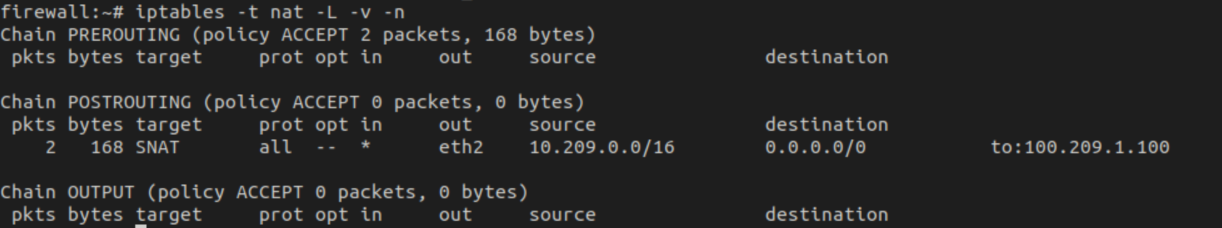
\includegraphics[width=0.8\textwidth]{ej2.1.3_5}
	\end{figure}
\end{enumerate}
\section{Servidores en la red privada, clientes externos}
Aunque en una red como la que aparece en la figura, lo habitual es colocar los servidores accesibles
desde el exterior en la zona DMZ, para ver cómo funciona DNAT, vamos a permitir que haya servidores
accesibles desde el exterior en la red privada interna.
\subsection{Apertura de puertos TCP}
Realiza un nuevo script \textbf{fw2.sh} en el firewall para que:
\begin{itemize}
	\item se borren las reglas que hubiera configuradas previamente en la tabla \textbf{nat}
	\item se reinicien los contadores de la tabla \textbf{nat}
	\item el tráfico de entrada al firewall destinado al puerto TCP 80 sea redirigido a \textbf{pc3}, puerto 80.
\end{itemize}
Incluye el script en la memoria. Ver el script en \ref{fw2}. Ejecuta dicho script y arranca las siguientes aplicaciones:
\begin{itemize}
	\item Inicia una captura en \textbf{r2(eth1)}(\textcolor{blue}{iptables-09.cap}) y en \textbf{r4(eth0)} (\textcolor{blue}{iptables-10.cap}).
	\item \textbf{nc }como servidor TCP en \textbf{pc3}, puerto 80
	\item \textbf{nc} como cliente TCP en \textbf{pc6}, de forma que su tráfico lo reciba el servidor de \textbf{pc3} (NOTA: presta
	especial atención a los parámetros con los que debes lanzar este cliente). Indica en la memoria el
	comando que has usado para lanzar el cliente y explica por qué lo has hecho así.\\
	
	He usado el comando: nc -p 6666 100.209.1.100 80.\\
	He usado esa Ip porque el firewall redirige automaticamente los mensajes que llegan a esa Ip y puerto a pc3 puerto 80, también porque si se lo envías a la dirección de pc3 los routers de internet no sabrán como redirigirlo.
	\item Escribe una palabra en el lado cliente y pulsa $<$Enter$>$
	\item Interrumpe la ejecución del cliente y el servidor.
	\item Interrumpe las capturas.
\end{itemize}
Explica los siguientes resultados:
\begin{enumerate}
	\item El resultado observado en \textbf{ip\_conntrack }y la traducción de direcciones IP y puertos realizada.\\
		
	Se puede observar en la imagen inferior que los datagramas enviados a la ip del router (100.209.1.100) con el puerto 80 son redirigidos a pc3 y al puerto 80.
	\begin{figure}[h]
		\centering
		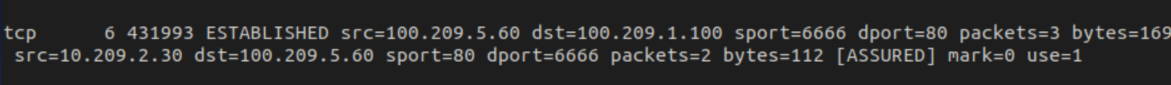
\includegraphics[width=0.8\textwidth]{ej2.2.1_1}
	\end{figure}
	\item La lista de reglas en el \textbf{firewall}, indica cuáles se están cumpliendo y cuántas veces.\\
	
	Se está cumpliendo la regla
	\begin{center}
		\begin{itemize}
			\item iptables -t nat -A PREROUTING -i eth2 -d 100.209.1.100 -p tcp --dport 80 -j DNAT --to-destination 10.209.2.30:80
		\end{itemize}
	\end{center}
	1 vez solo, ya que al ser una conexión Tcp solo se incrementará ese valor si se espera entre mensaje y mensaje 5 días.
	\begin{figure}[h]
		\centering
		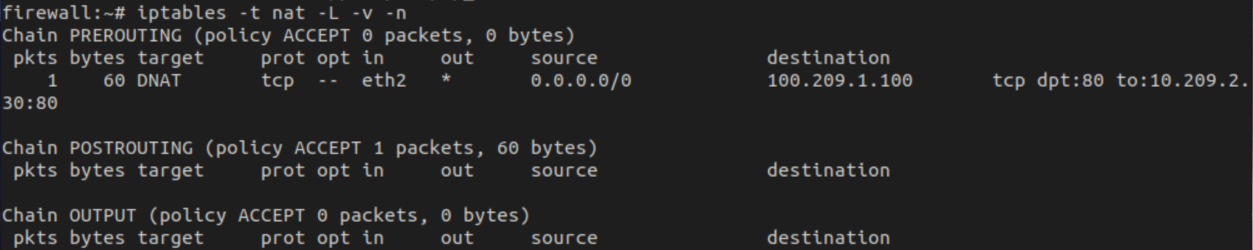
\includegraphics[width=0.8\textwidth]{ej2.2.1_2}
	\end{figure}
	\item Relaciona las reglas que se han cumplido con los datos de los mensajes capturados en los ficheros.\\
	
	En r2 se puede ver el intercambio de mensajes entre pc6 y pc3 con los datagramas que envía pc6 con la traducción ya hecha.\\
	Mientras que en r4 parece que el intercambio de mensajes es entre pc6 y el firewall como se puede ver en la siguiente imagen.\\
	\begin{figure}[h]
		\centering
		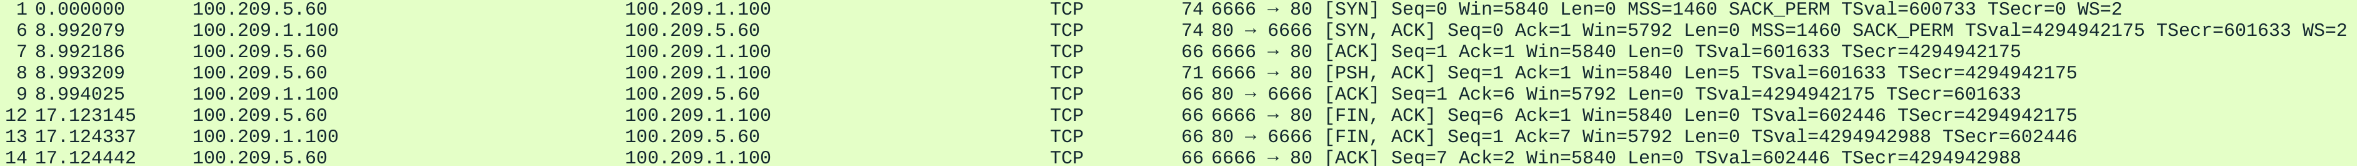
\includegraphics[width=0.9\textwidth]{ej2.2.1_3}
	\end{figure}
\end{enumerate}
\subsection{Apertura de puertos UDP}
Modifica el script \textbf{fw2.sh} para que, adicionalmente:
\begin{itemize}
	\item el tráfico de entrada al firewall destinado al puerto UDP 5001 sea redirigido a \textbf{pc1}, puerto 5001
	\item El tráfico de entrada al firewall destinado al puerto UDP 5002 sea redirigido a \textbf{pc2}, puerto 5001
\end{itemize}
Incluye el script en la memoria. Ejecuta el script que acabas de modificar y arranca las aplicaciones:
\begin{itemize}
	\item Inicia una captura en \textbf{r1(eth1)} (\textcolor{blue}{iptables-11.cap}), en \textbf{r4(eth0)} (\textcolor{blue}{iptables-12.cap}) y en \textbf{r5(eth1)} (\textcolor{blue}{iptables-13.cap}).
	\item \textbf{nc} como servidor UDP en \textbf{pc1}, puerto 5001
	\item \textbf{nc} como servidor UDP en \textbf{pc2}, puerto 5001
	\item \textbf{nc} como cliente UDP en \textbf{pc6}, de forma que su tráfico lo reciba el servidor de \textbf{pc1}. Indica el
	comando que has utilizado para lanzar el cliente y explica por qué.\\
	
	He usado el comando: nc -u -p 6666 100.209.1.100 5001.\\
	He usado esa Ip porque el firewall redirige automaticamente los mensajes que llegan a esa Ip y puerto a pc1 puerto 5001, también porque si se lo envías a la dirección de pc1 los routers de internet no sabrán como redirigirlo.
	\item \textbf{nc} como cliente UDP en \textbf{pc7}, de forma que su tráfico lo reciba el servidor de \textbf{pc2}. Indica el
	comando que has utilizado para lanzar el cliente y explica por qué.\\
	
	He usado el comando: nc -u -p 6666 100.209.1.100 5002.\\
	He usado esa Ip porque el firewall redirige automaticamente los mensajes que llegan a esa Ip y puerto a pc2 puerto 5001, también porque si se lo envías a la dirección de pc2 los routers de internet no sabrán como redirigirlo.
	\item Escribe una palabra en el lado cliente de \textbf{pc6} y \textbf{pc7} y pulsa $<$Enter$>$
	\item Interrumpe la ejecución de los clientes y servidores.
	\item Interrumpe las capturas.
\end{itemize}
Explica los siguientes resultados:
\begin{enumerate}
	\item El resultado observado en \textbf{ip\_conntrack }y la traducción de direcciones IP y puertos realizada.\\
	
	Se puede observar en la imagen inferior que los datagramas enviados a la ip del router (100.209.1.100) con el puerto 5001 son redirigidos a pc1 y al puerto 5001, mientras que los que van al puerto 5002 del firewall son redirigidos al puerto 5001 de pc2.
	\begin{figure}[h]
		\centering
		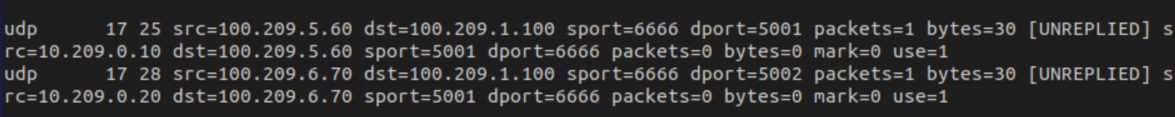
\includegraphics[width=0.8\textwidth]{ej2.2.2_1}
	\end{figure}
	\item Consulta la lista de reglas en el \textbf{firewall }e indica cuáles se están cumpliendo y cuántas veces.\\
	
	Se están cumpliendo las reglas
	\begin{center}
		\begin{itemize}
			\item iptables -t nat -A PREROUTING -i eth2 -d 100.209.1.100 -p udp --dport 5001 -j DNAT --to-destination 10.209.0.10:5001
			\item iptables -t nat -A PREROUTING -i eth2 -d 100.209.1.100 -p udp --dport 5002 -j DNAT --to-destination 10.209.0.20:5001
		\end{itemize}
	\end{center}
	1 vez cada una.
	\begin{figure}[h]
		\centering
		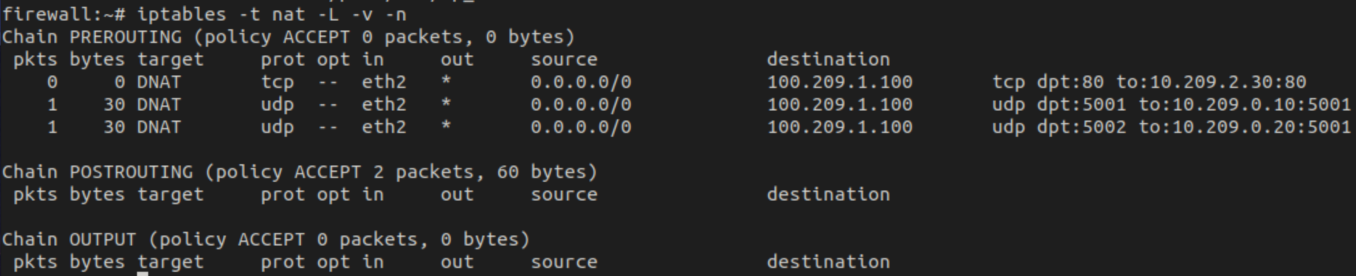
\includegraphics[width=0.8\textwidth]{ej2.2.2_2}
	\end{figure}
	\item Relaciona las reglas que se han cumplido con los datos de los mensajes capturados en los ficheros.\\
	
	En r1 se pueden ver los 2 mensajes con las direcciones traducidas.
	\begin{figure}[h]
		\centering
		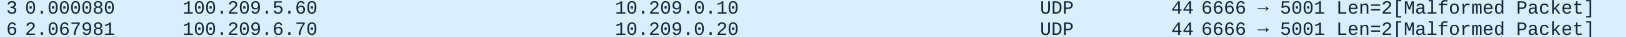
\includegraphics[width=0.9\textwidth]{ej2.2.2_3}
	\end{figure}\\
	Luego en r4 se ve el datagrama que envía pc6 a la dirección Ip del firewall que da a Internet y con el puerto 5001.\\
	Y por último en r5 se ve el datagrama que envía pc7 a la dirección Ip del firewall que da a Internet y con el puerto 5002.
\end{enumerate}
\chapter{Filtrado de tráfico en el \textit{firewall}: tabla filter}
Crea un \textit{script} \textbf{fw3.sh} en el \textbf{firewall} partiendo de la configuración de traducción de direcciones
realizada en \textbf{fw1.sh} (clientes en la red privada, servidores externos) al que se le añada la siguiente
configuración (todas en el mismo \textit{script}). Descripción de las \textbf{especificaciones}:
\begin{enumerate}
	\item Reiniciar la tabla \textbf{filter}: borrar su contenido y reiniciar sus contadores.
	\item Fijar las políticas por defecto de las cadenas de la tabla \textbf{filter}, haciendo que por defecto se
	descarte todo el tráfico en el \textbf{firewall} excepto los paquetes que cree el propio \textbf{firewall} (configuración habitual en un \textit{firewall} ).
	\item Permitir el tráfico de entrada dirigido a las aplicaciones que se están ejecutando en el propio
	\textbf{firewall} únicamente si este tráfico tiene su origen en las subredes privadas de la empresa.
	\item Permitir todo el tráfico saliente desde las subredes privadas hacia Internet y el tráfico de respuesta
	al saliente.\\
	
	Ten en cuenta que como has partido del \textit{script} \textbf{fw1.sh}, en dicho \textit{script} ya tenías las reglas de la
	tabla \textbf{nat} para la traducción de la dirección IP de origen de los paquetes que reenvía el \textbf{firewall}
	y los paquetes del tráfico entrante de respuesta a éste.
	\item Permitir desde Internet únicamente el tráfico entrante nuevo hacia la zona DMZ según las siguientes reglas:
	\begin{itemize}
		\item acceso a un servidor \textit{echo} existente en \textbf{pc4} (UDP, puerto 7). El servidor de \textit{echo} es un servidor
		que al enviarle una cadena de caracteres, devuelve la misma cadena que se le ha enviado.
		Para comprobar el acceso a este servidor utiliza \textbf{nc} como cliente desde otra máquina.
		\item acceso a un servidor \textit{daytime} existente en \textbf{pc5} (UDP, puerto 13). El servidor \textit{daytime} es un
		servidor que al enviarle algo, devuelve la fecha y hora de la máquina donde está instalado.
		Para comprobar el acceso a este servidor utiliza \textbf{nc} como cliente desde otra máquina.
	\end{itemize}
	Para este tipo de tráfico configura además regla/s con \textbf{acción LOG} para que cada vez que se
	permita el tráfico UDP descrito anteriormente, se deje un mensaje en el fichero de LOG del
	sistema.
	\item Permitir únicamente la comunicación entre la red privada y la zona DMZ de la siguiente forma:
	\begin{itemize}
		\item acceso desde \textbf{pc1} a un servidor de \textit{echo} (TCP, puerto 7) existente en \textbf{pc4}. En este caso,
		como todas las máquinas involucradas en la comunicación pertenecen al ámbito privado de
		la empresa, no es necesario que realices traducción de direcciones. Para este tipo de tráfico
		configura además regla/s con \textbf{acción LOG} para que cada vez que se permita este tráfico
		TCP, se deje un mensaje en el fichero de LOG del sistema.
	\end{itemize}
	\item Desde la zona DMZ \textbf{NO} se debe permitir iniciar ninguna comunicación con la red privada ni con
	el propio \textbf{firewall}.
\end{enumerate}
Incluye el script en la memoria. Ver el script en \ref{fw3}.\\

Prueba el resultado de la configuración del script:
\begin{enumerate}
	\item Sólo aplicaciones de la red privada pueden comunicarse con aplicaciones ejecutándose en el
	\textbf{firewall}:
	\begin{itemize}
		\item Ejecuta el script de configuración para que se reinicien los contadores.
		\item Prueba a lanzar un servidor TCP en el puerto 1111 de la máquina firewall. Lanza un cliente
		en \textbf{pc1} que se comunique con ese servidor. Indica qué reglas del firewall se están cumpliendo.\\
		
		Se esta cumpliendo la regla 
		\begin{center}
			iptables -t filter -A INPUT -i eth0 -j ACCEPT
		\end{center}
		2 veces, ya que es una comunicación Tcp.
		\begin{figure}[h]
			\centering
			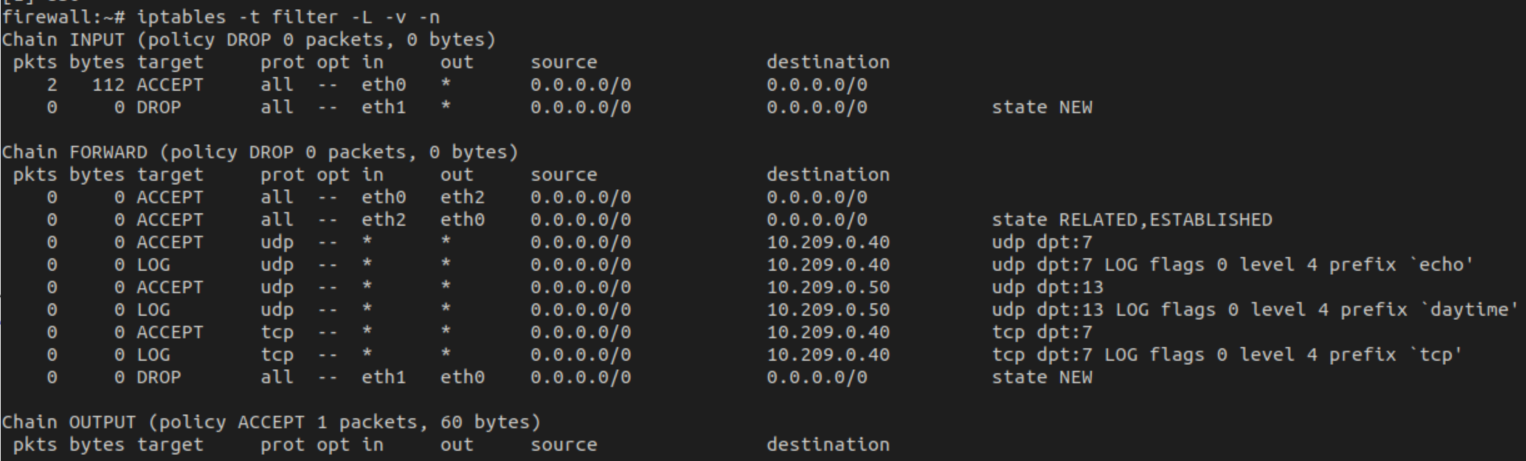
\includegraphics[width=0.8\textwidth]{ej3_1}
		\end{figure}
		\item Lanza un cliente en \textbf{pc6} que trate de comunicarse con ese servidor. Indica qué provoca que
		ese tráfico sea descartado.\\
		
		Porque pc6 al ser parte de la red no se le permite iniciar la conexión, ya que por defecto todos los mensajes que no cumplen las reglas se descartan.
	\end{itemize}
	\item Comunicación desde un cliente de la red privada con un servidor cualquiera en el exterior:
	\begin{itemize}
		\item Ejecuta el script de configuración para que se reinicien los contadores.
		\item Prueba a lanzar un servidor TCP en \textbf{pc6} en el puerto 1111. Realiza una captura de tráfico
		en \textbf{r3(eth0)} (\textcolor{blue}{iptables-14.cap}). Prueba a lanzar un cliente con \textbf{nc} desde \textbf{pc1} para que se
		comunique con este servidor.
		\item Consulta la lista de reglas en el \textbf{firewall} e indica cuáles se están cumpliendo y cuántas
		veces se cumplen como resultado de esta comunicación, tanto en la tabla nat como en la
		tabla filter.\\
				
		Se están cumpliendo las reglas
		\begin{center}
			\begin{itemize}
				\item iptables -t filter -A FORWARD -i eth0 -o eth2 -j ACCEPT
				\item iptables -t filter -A FORWARD -i eth2 -o eth0 -m state --state RELATED,ESTABLISHED -j ACCEPT
			\end{itemize}
		\end{center}
		2 veces la primera y 1 vez la segunda, mientras que en la tabla nat no se cumple ninguna.
		\begin{figure}[h]
			\centering
			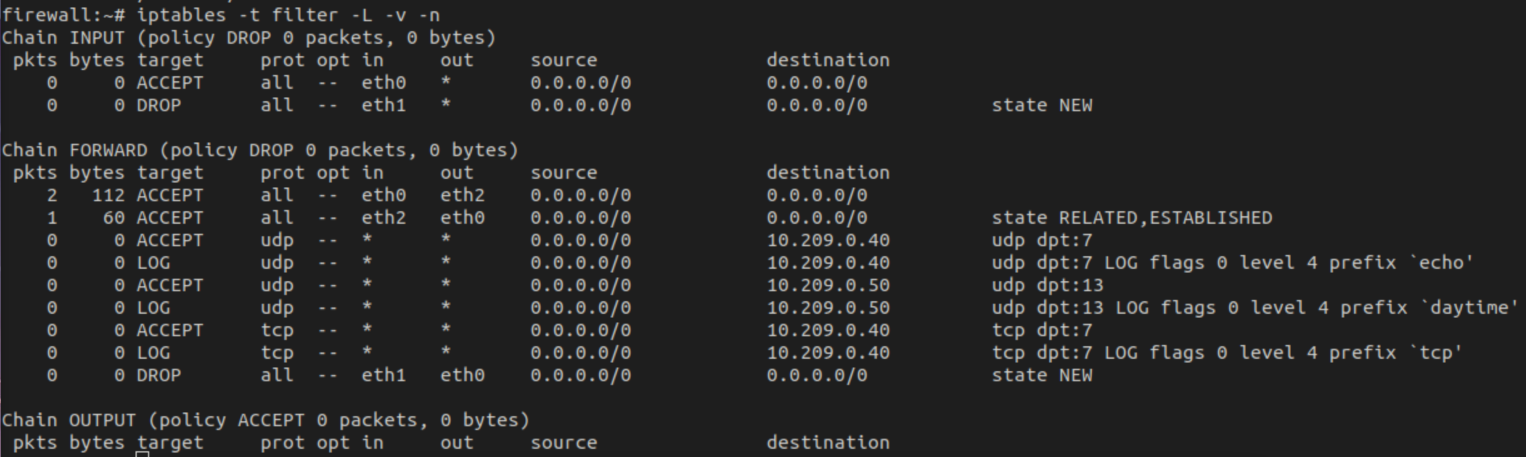
\includegraphics[width=0.8\textwidth]{ej3_2}
		\end{figure}
	\end{itemize}
	\item Comunicación entre \textbf{pc7} y servidor de UDP en el puerto 7 de \textbf{pc4}:
	\begin{itemize}
		\item Ejecuta el script de configuración para que se reinicien los contadores.
		\item En el escenario se encuentra lanzado en \textbf{pc4} un servidor UDP en el puerto 7 (\textit{echo}). Realiza
		una captura de tráfico en \textbf{pc4(eth0)} (\textcolor{blue}{iptables-15.cap}). Prueba a lanzar un cliente con
		nc desde \textbf{pc7} para que se comunique con este servidor.
		\item Consulta la lista de reglas en el \textbf{firewall} e indica cuáles se están cumpliendo y cuántas
		veces se cumplen como resultado de esta comunicación.\\
		
		Se estan cumpliendo las reglas
		\begin{center}
			\begin{itemize}
				\item iptables -t filter -A FORWARD -i eth2 -o eth1 -d 100.209.0.40 -p udp --dport 7 -j LOG --log-prefix echo
				\item iptables -t filter -A FORWARD -i eth2 -o eth1 -d 100.209.0.40 -p udp --dport 7 -j ACCEPT
			\end{itemize}
		\end{center}
		1 vez cada una, ya que la primera solo es el Log.
		\begin{figure}[h]
			\centering
			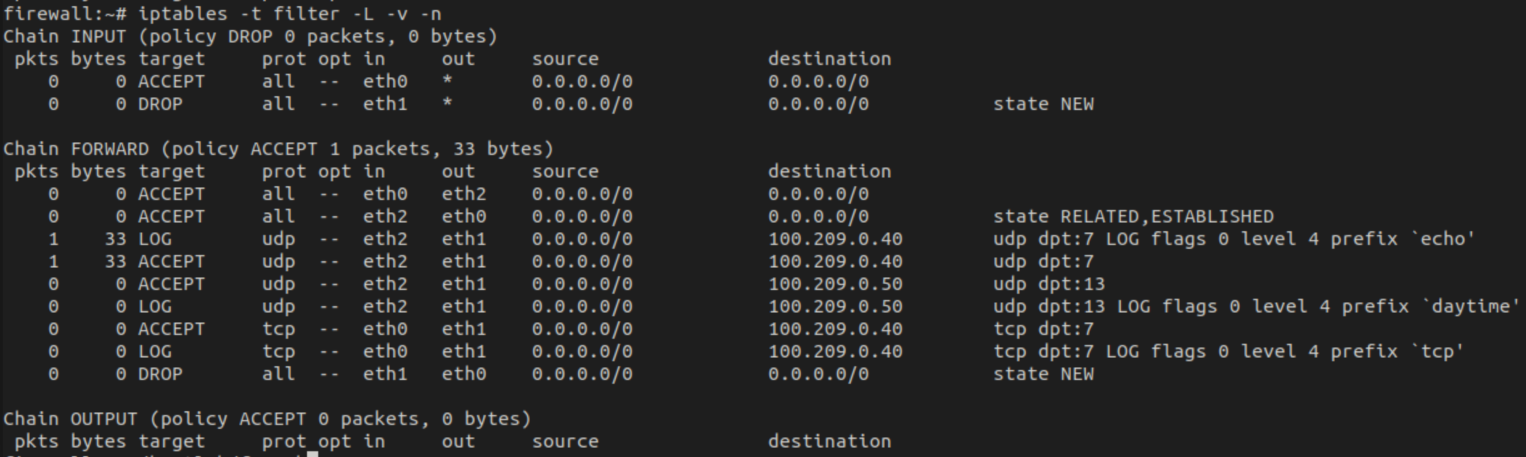
\includegraphics[width=0.8\textwidth]{ej3_3}
		\end{figure}
		\item Incluye en la memoria los mensajes que esta comunicación ha provocado en el fichero de
		log.\\
		
		Ver el log \ref{log3}.
	\end{itemize}
	\item Comunicación entre \textbf{pc6} y servidor de UDP en el puerto 13 de \textbf{pc5}:
	\begin{itemize}
		\item Ejecuta el script de configuración para que se reinicien los contadores.
		\item En el escenario se encuentra lanzado en \textbf{pc5} un servidor UDP en el puerto 13 (\textit{daytime}).
		Realiza una captura de tráfico en \textbf{pc5(eth0)} (\textcolor{blue}{iptables-16.cap}). Prueba a lanzar un cliente
		con \textbf{nc} desde \textbf{pc6} para que se comunique con este servidor.
		\item Consulta la lista de reglas en el \textbf{firewall} e indica cuáles se están cumpliendo y cuántas
		veces se cumplen como resultado de esta comunicación.\\
		
		Se estan cumpliendo las reglas
		\begin{center}
			\begin{itemize}
				\item iptables -t filter -A FORWARD -i eth2 -o eth1 -d 100.209.0.50 -p udp --dport 13 -j LOG --log-prefix daytime
				\item iptables -t filter -A FORWARD -i eth2 -o eth1 -d 100.209.0.50 -p udp --dport 13 -j ACCEPT
			\end{itemize}
		\end{center}
		1 vez cada una, ya que la primera solo es el Log.
		\begin{figure}[h]
			\centering
			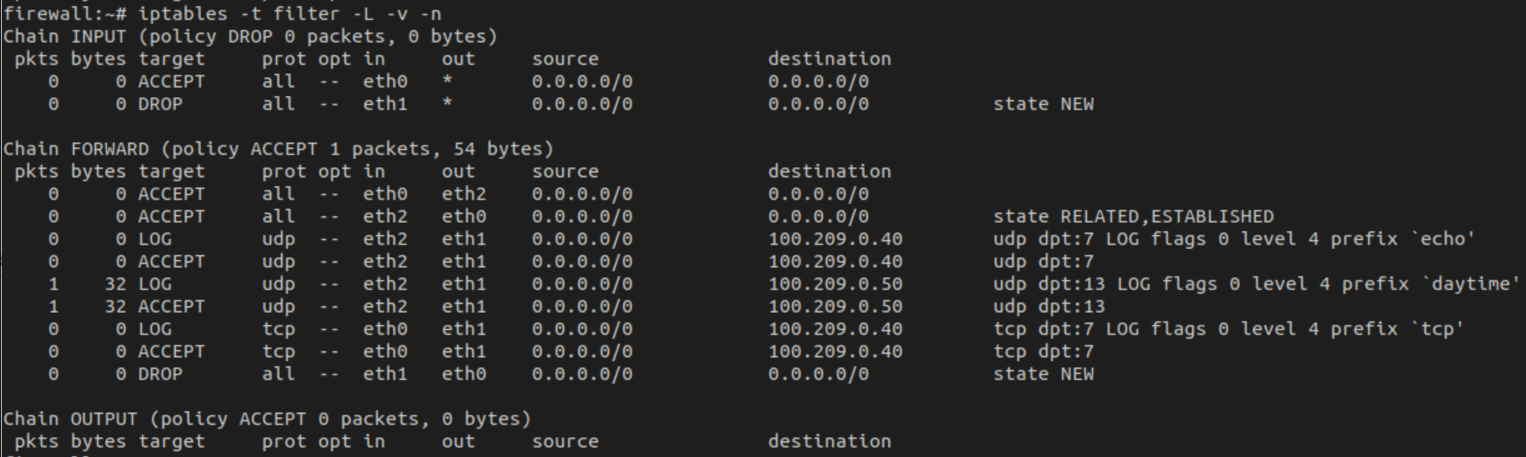
\includegraphics[width=0.8\textwidth]{ej3_4}
		\end{figure}
		\item Incluye en la memoria los mensajes que esta comunicación ha provocado en el fichero de
		log.\\
		
		Ver el log \ref{log4}.
	\end{itemize}
	\item Comunicación entre \textbf{pc1} y servidor de TCP en el puerto 7 de \textbf{pc4}:
	\begin{itemize}
		\item Ejecuta el script de configuración para que se reinicien los contadores.
		\item En el escenario se encuentra lanzado en \textbf{pc4} un servidor TCP en el puerto 7 (\textit{echo}). Realiza
		una captura de tráfico en \textbf{pc4(eth0)} (\textcolor{blue}{iptables-17.cap}). Prueba a lanzar un cliente con
		\textbf{nc} desde \textbf{pc1} para que se conecte con este servidor.
		\item Consulta la lista de reglas en el \textbf{firewall} e indica cuáles se están cumpliendo y cuántas
		veces se cumplen como resultado de esta comunicación. Es importante que observes que
		las reglas de la tabla \textbf{filter}, si se cumple la condición, se aplican con cada paquete que
		atraviesa el \textbf{firewall} y este comportamiento es diferente a lo que ocurría con las reglas de
		la tabla \textbf{nat}.\\
		
		Se estan cumpliendo las reglas
		\begin{center}
			\begin{itemize}
				\item iptables -t filter -A FORWARD -i eth0 -o eth1 -d 100.209.0.40 -p tcp --dport 7 -j LOG --log-prefix tcp
				\item iptables -t filter -A FORWARD -i eth0 -o eth1 -d 100.209.0.40 -p tcp --dport 7 -j ACCEPT
			\end{itemize}
		\end{center}
		6 veces cada una, ya que la primera solo es el Log. Como es una comunicación Tcp por cada intercambio de mensajes las reglas se cumplen 2 veces, al contrario que en la tabla nat, donde solo se aumenta el contador si pasan más de 5 días entre cada comunicación, es decir, en el ejemplo anterior solo se habría cumplido 1 norma 1 vez en vez de las 6 de la tabla filter.
		\begin{figure}[h]
			\centering
			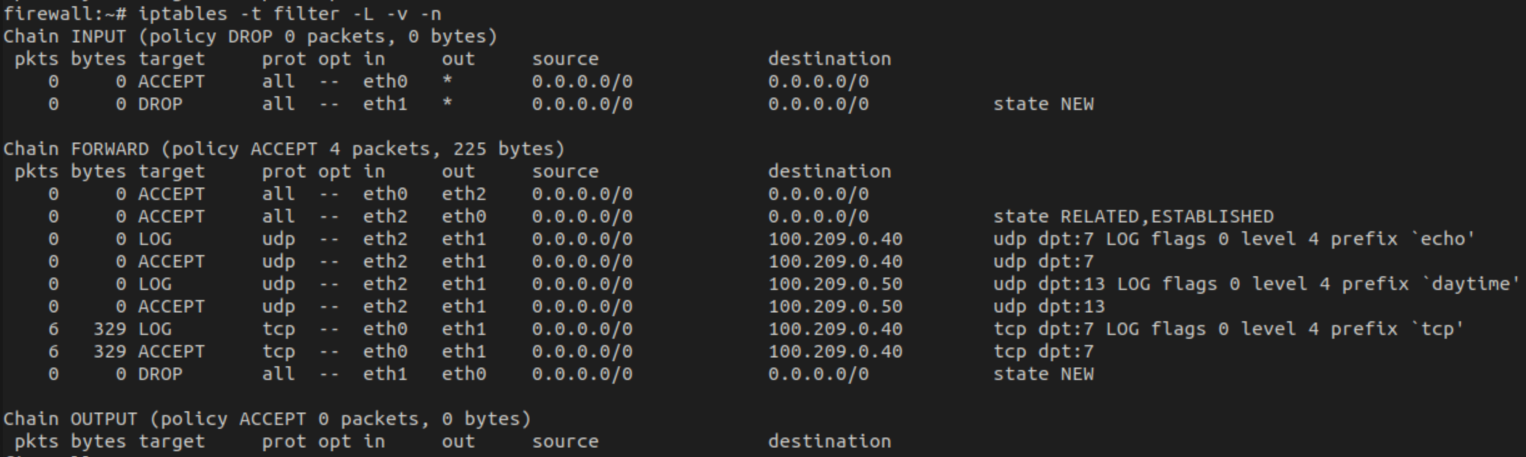
\includegraphics[width=0.8\textwidth]{ej3_5}
		\end{figure}
		\item Incluye en la memoria los mensajes que esta comunicación ha provocado en el fichero de
		log.\\
		
		Ver el log \ref{log5}.
	\end{itemize}
\end{enumerate}
\chapter{Scripts}
\lstinputlisting[caption=fw1.sh,language=Bash,basicstyle=\tiny,label=fw1]{include/fw1.sh}
\lstinputlisting[caption=fw2.sh,language=Bash,basicstyle=\tiny,label=fw2]{include/fw2.sh}
\lstinputlisting[caption=fw3.sh,language=Bash,basicstyle=\tiny,label=fw3]{include/fw3.sh}
\chapter{Logs}
\lstinputlisting[caption=Log 3.3,language=Bash,basicstyle=\tiny,label=log3]{include/log3_3.log}
\lstinputlisting[caption=Log 3.4,language=Bash,basicstyle=\tiny,label=log4]{include/log3_4.log}
\lstinputlisting[caption=Log 3.5,language=Bash,basicstyle=\tiny,label=log5]{include/log3_5.log}
\end{document}
